\subsection{Teorema Garis Bagi}
Misalkan garis bagi sudut $\angle A$ (bisa garis bagi dalam atau garis bagi luar) memotong garis $BC$ di $K$, maka 
$$\dfrac{BK}{CK} = \dfrac{AB}{AC}.$$
\begin{center}
    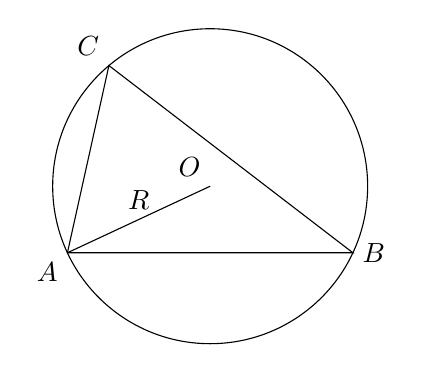
\begin{tikzpicture}
        \coordinate (O) at (0,0);
        \coordinate (B) at (-25:2cm);
        \coordinate (A) at (205:2cm);
        \coordinate (C) at (130:2cm);
        \coordinate (D) at (-90:2cm);
        
        \draw (O) circle (2cm);
        \draw (A) -- (B) -- (C) -- cycle;
        \node[right] at (B) {$B$};
        \node[below left] at (A) {$A$};
        \node[above left] at (C) {$C$};
        \node[above left] at (O) {$O$};
        \draw (A) -- node[above]{$R$} (O);
    \end{tikzpicture}
\end{center}